\documentclass[12pt, letterpaper, twoside]{article}
\usepackage[utf8]{inputenc}
\usepackage{graphicx}
\graphicspath{ {images/} }
 
\title{Practising Latex}
\author{Ayush Gupta}
\date{November 2017}

\begin{document}
\maketitle
This is the normal text we add to a \LaTeX{} file, devoid of any mathematical symbols. \\
You can also add some mathematical equations such as $3+5=8$, or some complex stuff as:
\begin{equation} [M]=e^{-\lambda t} \end{equation}
We can also change the size of fonts, and make it {\huge Big} or even very {\tiny tiny}\\
\section*{Graphs}
This is how you create a subsection in \LaTeX{}, and we have also eliminated the numbering which it provides automatically. 
\begin{figure}[h]
    \centering
    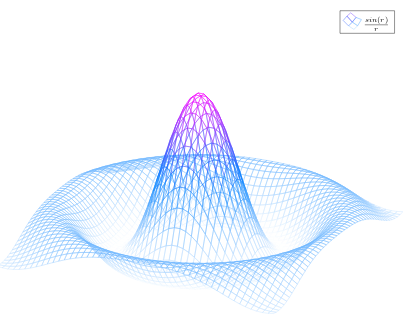
\includegraphics[width=0.25\textwidth]{mesh}
    \caption{A plot of $\frac{sin r}{r}$}
    \label{fig:mesh1}
\end{figure}
\paragraph{This is a basic Latex PDF Document}
\end{document}
